
\documentclass[letterpaper,hide notes,xcolor={table,svgnames},pdftex,10pt]{beamer}
\def\showexamples{t}

\usecolortheme{crane}
\setbeamertemplate{navigation symbols}{}

\usetheme{MyPittsburgh}
\usepackage{hyperref}
\usepackage{graphicx,xspace}
\usepackage[normalem]{ulem}
\usepackage{multicol}
\usepackage{amsmath,amssymb,amsthm,graphicx,xspace}
\newcommand\SF[1]{$\bigstar$\footnote{SF: #1}}

\usepackage[sfdefault,lf]{carlito}
\usepackage[T1]{fontenc}
\usepackage[scaled]{beramono}
\usepackage{tikzpagenodes}
\newcommand{\Rplus}{\protect\hspace{-.1em}\protect\raisebox{.35ex}{\small{\small\textbf{+}}}}
\newcommand{\Cpp}{\mbox{C\Rplus\Rplus}\xspace}

\newcounter{tmpnumSlide}
\newcounter{tmpnumNote}

\newcommand\mnote[1]{%
	\addtocounter{tmpnumSlide}{1}
	\ifdefined\showcues {~\tiny\fbox{\arabic{tmpnumSlide}}}\fi
	\note{\setlength{\parskip}{1ex}\addtocounter{tmpnumNote}{1}\textbf{\Large \arabic{tmpnumNote}:} {#1\par}}}

\newcommand\mmnote[1]{\note{\setlength{\parskip}{1ex}#1\par}}


\newcommand\mquestion[2]{{~\color{red}\fbox{?}}\note{\setlength{\parskip}{1ex}\par{\Large \textbf{?}} #1} \note{\setlength{\parskip}{1ex}\par{\Large \textbf{A}} #2\par}\ifdefined \presentationonly \pause \fi}

\newcommand\blackboard[1]{%
	\ifdefined   \showblackboard
		{#1}
	\else {\begin{center} \fbox{\colorbox{blue!30}{%
						\begin{minipage}{.95\linewidth}%
							\hspace{\stretch{1}} Some space intentionally left blank; done at the blackboard.%
						\end{minipage}}}\end{center}}%
	\fi%
}

\usepackage{listings}
\lstset{%
	keywordstyle=\bfseries,
	aboveskip=15pt,
	belowskip=15pt,
	captionpos=b,
	identifierstyle=\ttfamily,
	frame=lines,
	numbers=left, basicstyle=\scriptsize, numberstyle=\tiny, stepnumber=0, numbersep=2pt}

\usepackage{siunitx}
\newcommand\sius[1]{\num[group-separator = {,}]{#1}\si{\micro\second}}
\newcommand\sims[1]{\num[group-separator = {,}]{#1}\si{\milli\second}}
\newcommand\sins[1]{\num[group-separator = {,}]{#1}\si{\nano\second}}
\sisetup{group-separator = {,}, group-digits = true}

%% -------------------- tikz --------------------
\usepackage{tikz}
\usetikzlibrary{positioning}
\usetikzlibrary{arrows,backgrounds,automata,decorations.shapes,decorations.pathmorphing,decorations.markings,decorations.text}

\tikzstyle{place}=[circle,draw=blue!50,fill=blue!20,thick, inner sep=0pt,minimum size=6mm]
\tikzstyle{transition}=[rectangle,draw=black!50,fill=black!20,thick, inner sep=0pt,minimum size=4mm]

\tikzstyle{block}=[rectangle,draw=black, thick, inner sep=5pt]
\tikzstyle{bullet}=[circle,draw=black, fill=black, thin, inner sep=2pt]

\tikzstyle{pre}=[<-,shorten <=1pt,>=stealth',semithick]
\tikzstyle{post}=[->,shorten >=1pt,>=stealth',semithick]
\tikzstyle{bi}=[<->,shorten >=1pt,shorten <=1pt, >=stealth',semithick]

\tikzstyle{mut}=[-,>=stealth',semithick]

\tikzstyle{treereset}=[dashed,->, shorten >=1pt,>=stealth',thin]

\usepackage{ifmtarg}
\usepackage{xifthen}
\makeatletter
% new counter to now which frame it is within the sequence
\newcounter{multiframecounter}
% initialize buffer for previously used frame title
\gdef\lastframetitle{\textit{undefined}}
% new environment for a multi-frame
\newenvironment{multiframe}[1][]{%
	\ifthenelse{\isempty{#1}}{%
		% if no frame title was set via optional parameter,
		% only increase sequence counter by 1
		\addtocounter{multiframecounter}{1}%
	}{%
		% new frame title has been provided, thus
		% reset sequence counter to 1 and buffer frame title for later use
		\setcounter{multiframecounter}{1}%
		\gdef\lastframetitle{#1}%
	}%
	% start conventional frame environment and
	% automatically set frame title followed by sequence counter
	\begin{frame}%
		\frametitle{\lastframetitle~{\normalfont(\arabic{multiframecounter})}}%
		}{%
	\end{frame}%
}
\makeatother

\makeatletter
\newdimen\tu@tmpa%
\newdimen\ydiffl%
\newdimen\xdiffl%
\newcommand\ydiff[2]{%
	\coordinate (tmpnamea) at (#1);%
	\coordinate (tmpnameb) at (#2);%
	\pgfextracty{\tu@tmpa}{\pgfpointanchor{tmpnamea}{center}}%
	\pgfextracty{\ydiffl}{\pgfpointanchor{tmpnameb}{center}}%
	\advance\ydiffl by -\tu@tmpa%
}
\newcommand\xdiff[2]{%
	\coordinate (tmpnamea) at (#1);%
	\coordinate (tmpnameb) at (#2);%
	\pgfextractx{\tu@tmpa}{\pgfpointanchor{tmpnamea}{center}}%
	\pgfextractx{\xdiffl}{\pgfpointanchor{tmpnameb}{center}}%
	\advance\xdiffl by -\tu@tmpa%
}
\makeatother
\newcommand{\copyrightbox}[3][r]{%
	\begin{tikzpicture}%
		\node[inner sep=0pt,minimum size=2em](ciimage){#2};
		\usefont{OT1}{phv}{n}{n}\fontsize{4}{4}\selectfont
		\ydiff{ciimage.south}{ciimage.north}
		\xdiff{ciimage.west}{ciimage.east}
		\ifthenelse{\equal{#1}{r}}{%
			\node[inner sep=0pt,right=1ex of ciimage.south east,anchor=north west,rotate=90]%
			{\raggedleft\color{black!50}\parbox{\the\ydiffl}{\raggedright{}#3}};%
		}{%
			\ifthenelse{\equal{#1}{l}}{%
				\node[inner sep=0pt,right=1ex of ciimage.south west,anchor=south west,rotate=90]%
				{\raggedleft\color{black!50}\parbox{\the\ydiffl}{\raggedright{}#3}};%
			}{%
				\node[inner sep=0pt,below=1ex of ciimage.south west,anchor=north west]%
				{\raggedleft\color{black!50}\parbox{\the\xdiffl}{\raggedright{}#3}};%
			}
		}
	\end{tikzpicture}
}


%% --------------------

%\usepackage[excludeor]{everyhook}
%\PushPreHook{par}{\setbox0=\lastbox\llap{MUH}}\box0}

%\vspace*{\stretch{1}

%\setbox0=\lastbox \llap{\textbullet\enskip}\box0}

\setlength{\parskip}{\fill}

\newcommand\noskips{\setlength{\parskip}{1ex}}
\newcommand\doskips{\setlength{\parskip}{\fill}}

\newcommand\xx{\par\vspace*{\stretch{1}}\par}
\newcommand\xxs{\par\vspace*{2ex}\par}
\newcommand\tuple[1]{\langle #1 \rangle}
\newcommand\code[1]{{\sf \footnotesize #1}}
\newcommand\ex[1]{\uline{Example:} \ifdefined \presentationonly \pause \fi
	\ifdefined\showexamples#1\xspace\else{\uline{\hspace*{2cm}}}\fi}

\newcommand\ceil[1]{\lceil #1 \rceil}


\AtBeginSection[]
{
	\begin{frame}
		\frametitle{Outline}
		\tableofcontents[currentsection]
	\end{frame}
}



\pgfdeclarelayer{edgelayer}
\pgfdeclarelayer{nodelayer}
\pgfsetlayers{edgelayer,nodelayer,main}

\tikzstyle{none}=[inner sep=0pt]
\tikzstyle{rn}=[circle,fill=Red,draw=Black,line width=0.8 pt]
\tikzstyle{gn}=[circle,fill=Lime,draw=Black,line width=0.8 pt]
\tikzstyle{yn}=[circle,fill=Yellow,draw=Black,line width=0.8 pt]
\tikzstyle{empty}=[circle,fill=White,draw=Black]
\tikzstyle{bw} = [rectangle, draw, fill=blue!20,
text width=4em, text centered, rounded corners, minimum height=2em]

\newcommand{\CcNote}[1]{% longname
	This work is licensed under the \textit{Creative Commons #1 3.0 License}.%
}
\newcommand{\CcImageBy}[1]{%
	\includegraphics[scale=#1]{creative_commons/cc_by_30.pdf}%
}
\newcommand{\CcImageSa}[1]{%
	\includegraphics[scale=#1]{creative_commons/cc_sa_30.pdf}%
}
\newcommand{\CcImageNc}[1]{%
	\includegraphics[scale=#1]{creative_commons/cc_nc_30.pdf}%
}
\newcommand{\CcGroupBySa}[2]{% zoom, gap
	\CcImageBy{#1}\hspace*{#2}\CcImageNc{#1}\hspace*{#2}\CcImageSa{#1}%
}
\newcommand{\CcLongnameByNcSa}{Attribution-NonCommercial-ShareAlike}

\newenvironment{changemargin}[1]{% 
	\begin{list}{}{% 
		\setlength{\topsep}{0pt}% 
		\setlength{\leftmargin}{#1}% 
		\setlength{\rightmargin}{1em}
		\setlength{\listparindent}{\parindent}% 
		\setlength{\itemindent}{\parindent}% 
		      \setlength{\parsep}{\parskip}% 
		      }% 
		\item[]}{\end{list}}





\title{Lecture 13 --- Thread Implementation }

\author{Jeff Zarnett \& Mike Cooper-Stachowsky \\ \small \texttt{jzarnett@uwaterloo.ca, mstachowsky@uwaterloo.ca}}
\institute{Department of Electrical and Computer Engineering \\
  University of Waterloo}
\date{\today}
\begin{document}

\begin{frame}
  \titlepage
\end{frame}


\begin{frame}
\frametitle{Make it So}

With the thread theory behind us, now we need to actually work with some.

\begin{center}
	
\includegraphics[width=0.3\textwidth]{images/making-it-so.jpg}
\end{center}

The model we'll use is a bit simpler than the UNIX thread (but we'll get there).

\end{frame}


\begin{frame}
\frametitle{How To Get Started}

A thread runs code and has some function that it starts with...\\
\quad Like \texttt{main()} in C, but it can be named anything.

There must be a way of keeping track of where we are in the execution.

We also need a stack for each thread (so a stack pointer).

\end{frame}


\begin{frame}[fragile]
\frametitle{Starting a Thread}

Thread functions all have the same prototype:

\begin{lstlisting}[language=C]
void * function_name( void * argument ) {
  /* Interpret the argument(s) as needed here */
 
  /* Many threads never return, so they just loop forever as needed */ 
}
\end{lstlisting}

Why \texttt{void *} for input and output?

\end{frame}


\begin{frame}
\frametitle{Anything Goes}

The OS designer can't know what input and output an arbitrary thread will have.

So let the programmer choose! \texttt{void *} means it can be anything.

\begin{center}
	
\includegraphics[width=0.5\textwidth]{images/reality.png}
\end{center}

\end{frame}


\begin{frame}
\frametitle{I'll Show Myself Out}

Threads rarely exit in a real-time operating system.\\
\quad Generally it's a continuous-operation system doing specific things.


You can make the return type \texttt{void} in your OS, but it's not 100\% correct.

More correct: exit from a thread is a system call, and tells the OS this thread cannot run ever again.

\end{frame}



\begin{frame}
\frametitle{Starting the New Thread}

If we've defined the starting function, can we just... call it?

No; that would run it in the \textit{current} thread.

\begin{center}
	
\includegraphics[width=0.5\textwidth]{images/doitmyself.png}
\end{center}

We need to run it as a new thread instead. 

\end{frame}


\begin{frame}
\frametitle{It's like Delegation}

\begin{center}
	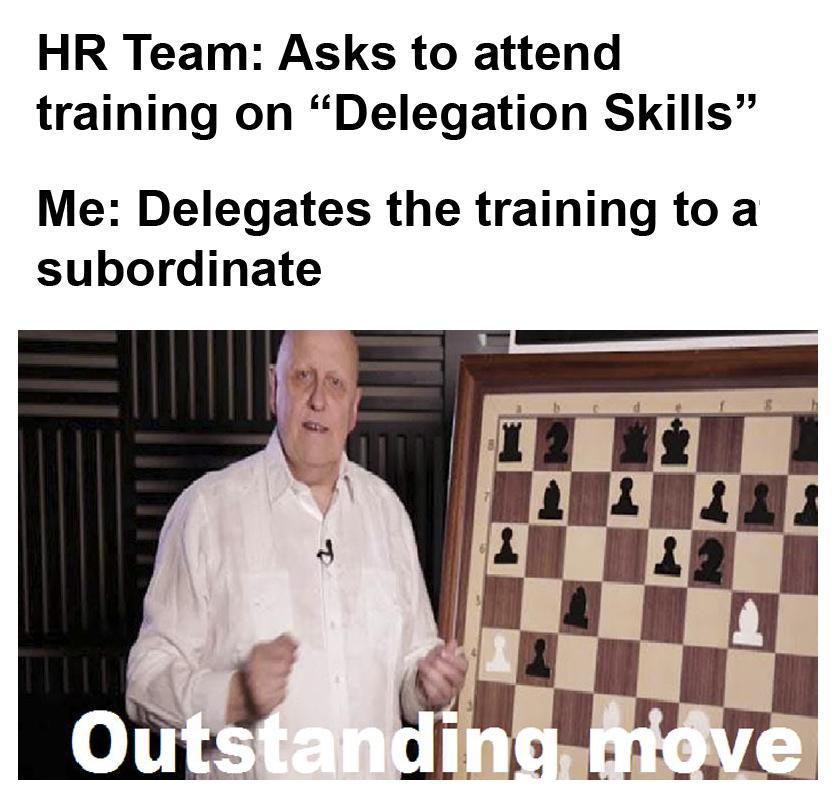
\includegraphics[width=0.4\textwidth]{images/delegate2.jpg}
\end{center}

In addition to the code to run, we need a new stack and the thread context.

\end{frame}


\begin{frame}
\frametitle{Context}

Context is the data a thread needs while running.

Obvious example: keep track of progress in the code!

But also: register data and stack pointer.

In a bigger OS: maybe permissions, open files, etc.

\end{frame}



\begin{frame}
\frametitle{Own Stack}

Remember: the stack is local storage for each thread...\\
\quad And also the execution trace to how we got here.

If we had one shared stack for everyone, all threads write to it. 

Overwrite each other's data, overlapping execution traces...
\begin{center}
	
\includegraphics[width=0.4\textwidth]{images/chaoselmo.jpg}
\end{center}

\end{frame}


\begin{frame}
\frametitle{Where to Thread Stacks Come From?}

So if a thread needs a stack, where does it come from?

The OS can just designate an area of memory as the stack for a given thread.

\begin{center}
	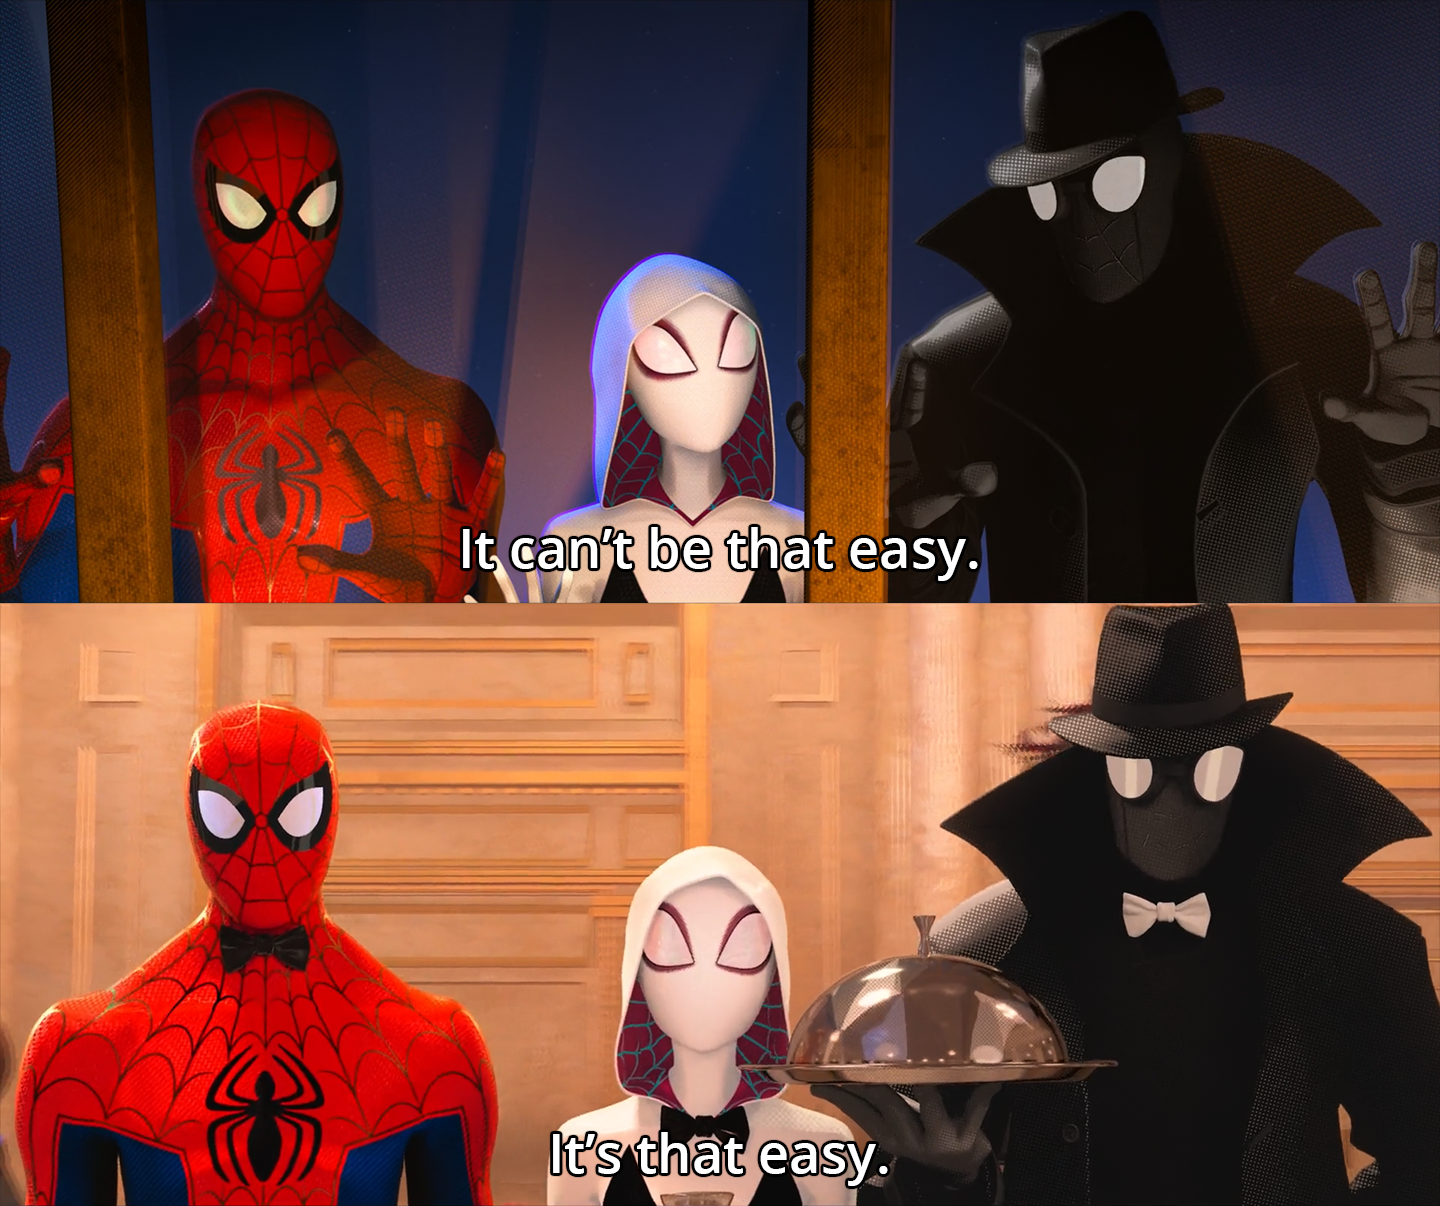
\includegraphics[width=0.5\textwidth]{images/thateasy.png}
\end{center}


You could divide the OS stack into different pieces, one for each thread.
\end{frame}



\begin{frame}
\frametitle{Stack Pool}

If each thread gets a piece of the OS stack, can they overwrite each other if one of the stacks gets too big?

Yes (unless we have virtual memory or similar). So on the Cortex M... yes.

This sort of stack overflow can corrupt data, and can't be prevented.\\
\quad We just say it's the application programmer's problem.

\end{frame}


\begin{frame}
\frametitle{Minimal Thread Control Block}

We covered the idea of the process control block fairly thoroughly. 

A minimal thread control block (TCB) has:

\begin{itemize}
	\item Identifier
	\item Instruction pointer
	\item Stack pointer
\end{itemize}

We may or may not have the starting point of the thread in there.

\end{frame}


\begin{frame}
\frametitle{Context is Not Data}

Context is not entirely the same as the data.

Context is how we know what we're doing and where we are.

Data is things that a thread needs to do its job.


\end{frame}


\begin{frame}
\frametitle{Corruption}

If our context gets corrupted we'll crash (hard fault) very quickly.

If the data is corrupted, the output is wrong or garbage...\\
\quad We may get a hard fault, but not necessarily.

\begin{center}
	
\includegraphics[width=0.5\textwidth]{images/wronganswer.jpg}
\end{center}

\end{frame}



\begin{frame}
\frametitle{Take Turns}

For threads to take turns on the CPU, it means we have to save and load their context information. 

When thread A's context is loaded, it can run.

When its turn is over, save the context, and load that of thread B.

... Now generalize that to arbitrarily many threads.


\end{frame}


\begin{frame}
\frametitle{Whose Turn is it Anyway?}

\begin{center}
	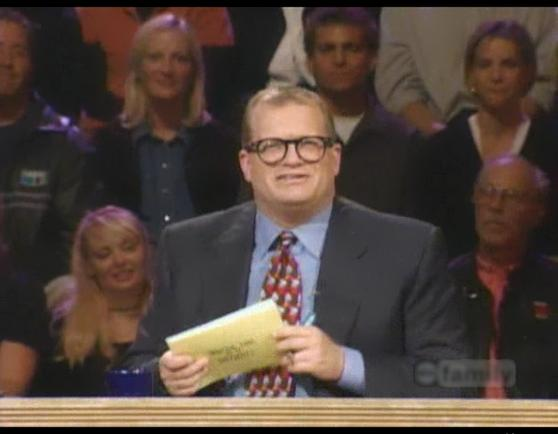
\includegraphics[width=0.3\textwidth]{images/whoseturn.jpg}
\end{center}

That's a scheduling decision, so we'll come back to that soon.


\end{frame}


\begin{frame}
\frametitle{Setting up a Thread}

\begin{enumerate}
	\item Create the TCB.
	\item Designate some area of memory to be the stack.
	\item Set up the stack to contain the context of the thread.
	\item The Kernel must:
		\begin{itemize}
			\item Set \texttt{xPSR} to \texttt{1<<24} (trust us)
			\item Set \texttt{PC} to the thread's function pointer
			\item Put input argument into \texttt{R0}
			\item Put the stack \texttt{16x4} bytes down from \texttt{xPSR}
			\item Store in order: \texttt{xPSR, PC, LR, R12, R3, R2, R1, R0, R11} through \texttt{R4}
		\end{itemize}
\end{enumerate}


\end{frame}


\begin{frame}
\frametitle{That Seems Complicated}

\begin{center}
	
\includegraphics[width=0.4\textwidth]{images/ytho.jpg}
\end{center}

The goal is to make it seem to the chip like the thread has already run.

We are setting up the thread context on the stack just like it would be saved.

If you forgot something (likely) you'll get a hard fault.

\end{frame}


\begin{frame}
\frametitle{What was I doing again?}

We have been circling around the idea of the context switch a lot so far.

It may make conceptual sense but maybe unclear on how to implement it.\\
\quad This is what labs 2 and 3 are for.

Context switch is a very hard part of OS development...\\
\quad And any bug in it will be a huge problem!

\end{frame}


\begin{frame}
\frametitle{Managing this in a RTOS}

If there are many TCBs to manage, do they go in a list or array? Design decision!

The OS needs its own stack pointer (use \texttt{MSP}).

It also needs to keep track of how many threads exist, what's running now, and how much stack space is available to allocate.


\end{frame}


\begin{frame}
\frametitle{Basic Functionality}

The RTOS needs to be able to:

\begin{itemize}
	\item Initialize itself
	\item Create a new thread
	\item Start running a thread
	\item Switch between threads
\end{itemize}

\begin{center}
	
\includegraphics[width=0.4\textwidth]{images/fancy.jpg}
\end{center}


\end{frame}


\begin{frame}[fragile]
\frametitle{Function Prototypes}

\begin{lstlisting}[language=C]
kernelInit( ... ); // Initialize kernel data and chip settings

osCreateThread( ... ); // Make a new thread and register it with the kernel

kernelStart( ... ); // Run the first thread

osSched( ... ); // Run scheduler (choose new thread to run)

osYield( ... ); // Voluntarily give up the CPU, tell the scheduler to run

\end{lstlisting}

Initialization function: set kernel variables, set interrupt priority, create TCBs, create stack pointers.

Create Thread: get a new stack (fail if no space), initialize the thread stack, update OS variables to track new thread.

\end{frame}


\begin{frame}
\frametitle{Abut Scheduling}

Scheduling is so complex it gets its own section of the course (next one!).

Key question: which thread gets to run when?

In the labs, we use Round Robin until Lab 5.

\end{frame}


\begin{frame}
\frametitle{Terminating a Thread}

In our simple OS a thread that just... ends... will cause a hard fault.

It can be done! Remove the thread from scheduling; deallocate its resources.

That has to happen in a bigger OS (UNIX); otherwise we're leaking memory.


\end{frame}


\begin{frame}
\frametitle{To Boldly Go...}

\begin{center}
	
\includegraphics[width=0.5\textwidth]{images/setcourse.jpg}
\end{center}

Well then, let's get on to what threads are like in UNIX.

\end{frame}



\end{document}

